\chapter{基于弱监督注意力的多人姿态估计方法}
\label{cha:method}

\section{概述}
\label{sec:methodoverview}
%   This part intends to state the overall idea
%	ROI Extraction
%	key-point & Mask Prdiction
%		Stage One's Prediction
%		Stage 2+'s Prediction
Our method uses ResNet-101 as backbone of our network and FPN as our feature extraction module. The structure can be divided into two sections: the detection section, which predicts the bounding box positions, coarse key-points and mask predictions, and the refine section which extracts and improve the key-point and instance segmentation prediction. Specifically, in the refine section, the network use a multi-stage architecture where key-points and masks are both involved. The architecture was inspired by the attention mechanism. This method managed to use attention mechanism to help the network focus on specific spatial area to give more accurate prediction, and even more, an instance segmentation that contains more information, for example the occluded parts.\\
The feature maps from the extractor are divided into two copies. The first copy is consumed by a group of shared convolution layers, concatenated with $K_{t-1}$ from $stage_{t-1}$ as the input of those layers. The second copy flows to the \textit{Attention Converter} module, also is concatenated with $M_{t-1}$ from $stage_{t-1}$.To get refined key-point predictions, the \textit{key-point head} takes feature maps which are multiplied by soft attention from the \textit{Attention Converter}. On the other hand, the mask prediction accept both attention and features from the \textit{share conv}. As the refine stage takes mask and key-point prediction from last stage and output for the current stage, we can denote the refine stage as \eqref{def:refinenet}, where $R$ refers the refine stage.
\begin{equation}
\label{def:refinenet}
M_t, K_t = R(M_{t-1}, K_{t-1})
\end{equation}
	%   This part is to describe why we use a hybrid multi-stage arch
%	1. mask and key-point detection is associated
%	2. In crowd, the heatmap is not robust to predict
Our method employs a multi-staged architecture with weakly supervised feature-level attention to refine the prediction of both the human pose and the instance segmentation. Firstly, we think that predicting an instance segmentation of a person and its key-points are associated tasks. The key-point detection result can be refined by masks. Also, the key-point detection stage in crowded scene is not robust, which means the network will be interfere by the person around the center. Hence, our method adopted an iterative refinement structure, applying attention mechanism to help the network focus on specific target. Furthermore, multi-staged architecture provides larger reception field to both key-point and mask branch, which strengthen the network's ability on distinguishing different instances.

\section{人体位置与姿态粗检测阶段}
\label{sec:detectionstage}
%	Structure description
%	1. Hybrid arch of maskrcnn & cpm
Our method managed to use a hybrid model in the detection section. ResNet-101 with FPN generates RoIs in multiple scales. After paralleled RPN consuming feature from different size, we applied pyramid RoI align layer to produce feature maps regarding to the object's size. Regression head is designed here to output accurate bounding boxes which help mask and key-point branch to generate coarse predictions. The mask and key-point branch are paralleled in the architecture. Coarse mask branch uses 4 convolution layers with kernel size of 3, followed by a transposed convolution layer with stride 2 and kernel size 2.

\begin{figure*}[htbp]
	\centering
	\includegraphics[scale=0.65]{RefineNet.pdf}
	\caption{Details of RefineNet}
	\label{fig:RefineNet}
\end{figure*}

%   Training strategy description
%	Section 1
In the training process, as we designed the network into two sections, the global loss function is also defined as a combination of two separated loss \eqref{detection_loss}. For the first section we train the network to learn how to extract instance positions, coarse mask and key-point predictions. So we defined the loss function in a R-CNN fashion, calculating distance between prediction confidence and labels using cross entropy over softmax gate. To train the network to predict coarse mask, a cross entropy is also defined here to get masks of three classes \eqref{bbox_mask_loss}. And the loss in key-point branch is defined as naive mean square error function \eqref{coarse_key-point_loss}.

\begin{equation}
%	section 1 loss
\label{detection_loss}
L_{detection} = L_{bbox\&mask_{reg}} + L_{key-point_{reg}}
\end{equation}      
\begin{equation}
%	bbox & mask regression loss
\label{bbox_mask_loss}
L_{bbox\&mask_{reg}} = -\sum_{c \in C}{\hat{p_c} \log{p_c^{*}}}  -\sum_{c \in C}{\hat{m_c} \log{m_c^{*}}}
\end{equation}
\begin{equation}
%	coarse mask regression loss
\label{coarse_key-point_loss}
L_{key-point_{reg}} = -\sum_{i \in I}\sum_{k \in K}{\left\| \hat{k_i} - {k_i}^{*} \right\|_2}
\end{equation}


\section{融合阶段}
\label{sec:refine}
\subsection{网络结构}
\label{subsec:architecture}
%	TODO: more detailed content to discuss the net structure in refine section
%	1. What the network looks like
%	2. Why we propose the network like this? (need to be explain by experiments)
%		a) training process (featured points)
%			(i)		loss penalty calculation
%		b) inference process 
%			(i)		attention-like instance segmentation
%Size of reception field is crucial to the refine section, as the key-point branch need them to avoiding the wrong decision in 
The refine section is divided into 5 seperated stages, and each part can be denoted as equation\eqref{def:refinenet}, to be more in detail, the network can be defined as below:
\begin{equation}
c = C({f}\otimes{K_{t-1}})
\end{equation}
\begin{equation}
a = A(f\otimes{M_{t-1}})
\end{equation}
\begin{equation}
K_t = H_k(c\odot a)
\end{equation}
\begin{equation}
M_t = H_m(F(c) \oplus a)
\end{equation}
where $\otimes$ refers to concatenating operation, $\odot$ for bit-wise multiply, and $\oplus$ is for bit-wise add operation. $M_t$ and $K_T$ denote the mask and key-point prediction from stage $t$. The feature map is denoted as $f$, and $a$ is for attention, $c$ is for the output from the shared convolution layers. In notations for modules, $C$ is for shared convolution layers, $A$ is for attention converter, and $F$ is for the fusion module. $H_k$ is for the key-point head, and the $H_m$ is for mask head.\\
It is common to generate attention using a given feature from last stage, and we suppose that the instance segmentation prediction, still can be treated as a strong cue to the soft attention. Therefore, our method proposed a attention converter to digest features and mask prediction from last stage to generate proper attention to the network.\\
However, the attention may be incompatible for a multi-staged architecture to supervise. Hence, a single layered mask head is designed here to adjust the dimension to the binary mask, which makes it easier to define losses to the attention. In another hand, like other the traditional multi-tasking networks, our method also employs a separated head which accepts features from a shared convolution to use the common priors which are used by the key-point prediction. To hybrid those two idea in the design of networks, we proposed the refine stage which is shown in Fig.\ref{fig:RefineNet}.\\

\subsection{损失函数定义}
\label{subsec:lossfunctions}
%	Section 2 Training
%	key-point Loss
%	Why Applying masks after 1x1 conv?
%	1.	explicitly define loss with mask & key-points
%	2.	simply enhance response of the heatmap
%		rather than enhance the result
%			--> This will give more responses
%	TODO: quote attention paper to prove it
Training strategy in section 2 is divided into two parts: key-point branch loss and instance segmentation loss. Loss in section 2 can be defined as a summing function from the second stage to the last \eqref{total_refine_loss}, where $\alpha$ is 0.05.

%	TODO: fit the <Attention is all you need> thread into this section
Training key-point branch is similar to the process in section 1. We define MSE loss to measure errors between ground truth and prediction. But what is different in section 2 is that the key-point predictions are affected by the instance mask implicitly, as we multiply them with those masks in a bit-wise fashion before 1x1 convolution layers. The 1x1 convolution layers will not change the size of reception field, therefore the operation we perform here are nearly the same as multiplying after the network. But with those trainable parameters in 1x1 convolution layers, the network will need no explicit definition of any masks in loss function of the key-point branch and also can strengthen the response at relative positions on feature maps. This is intended to avoid multiplying zeros on the result in key-point branch, which causes failure on supervising both key-point prediction and instance segmentation with one loss. The loss function in key-point branch $L_{k_t}$ where $t>1$ is defined as \eqref{refine_key-point_loss}. 

%	Total Refine Loss
\begin{equation}
\label{total_refine_loss}
L_{refine} = \sum_{t=2}^{T}{L_{k_t} + \alpha L_{m_t}}
\end{equation}

%	Refine key-point Loss
\begin{equation}
\label{refine_key-point_loss}
L_{k_{t}} = -\sum_{i \in I}\sum_{j \in J}{\parallel \hat{k_i} - {k_i}^{*} \parallel_2}
\end{equation}

%	Instance segmentation supervision
%	Localization loss
%		smoothed L1
%			attention-like
%	TODO: More attention paper quotations
Supervising mask branch is a more complicated process, because we want to train the network in order to complete the losing part where the detection section failed to infer. Therefore we consider to calculate both localization error and overlap penalty \eqref{mask_loss} for stage $t$ where $t>1$. We set the $beta$ in equation\eqref{mask_loss} to 0.2. The localization error is defined as \eqref{mask_loc_loss}. Instead applying a cross entropy loss here, we introduce smoothed L1 loss here, as the network use instance segmentation as attention.

%	Mask Loss
%	Semi supervision
\begin{equation}
\label{mask_loss}
L_{m_t}=L_{loc_t} - \beta L_{ins\ penalty_t}
\end{equation}

\begin{equation}
\label{mask_loc_loss}
L_{loc}^t =  \sum_{p \in P} Smooth_{L1}( H^{p}_{gt} - H^{p}_{pred} )
\end{equation}

\subsection{训练策略}
\label{subsec:trainingstrategy}
%	TODO: Training Strategy
%	Training Setups
%		learning rate
%		optimizer
%		separated trained ( sec 1 -> sec 2)
We use a two-stage separated training strategy. In the first stage, we train the joint branch only at learning rate of 4e-4 (all stages) for 60 epochs, with the epoch size of 1000 and the exponential learning rate decay (0.333 every 20 epoch). In the second stage, we train the whole refine branch with the total Loss, which equals to refine joint loss plus refine mask loss multiply by ten, with the base lr 1e-4 with exponential decay of 0.333 every 30 epoch.


\begin{figure}[htbp]
	\centering
	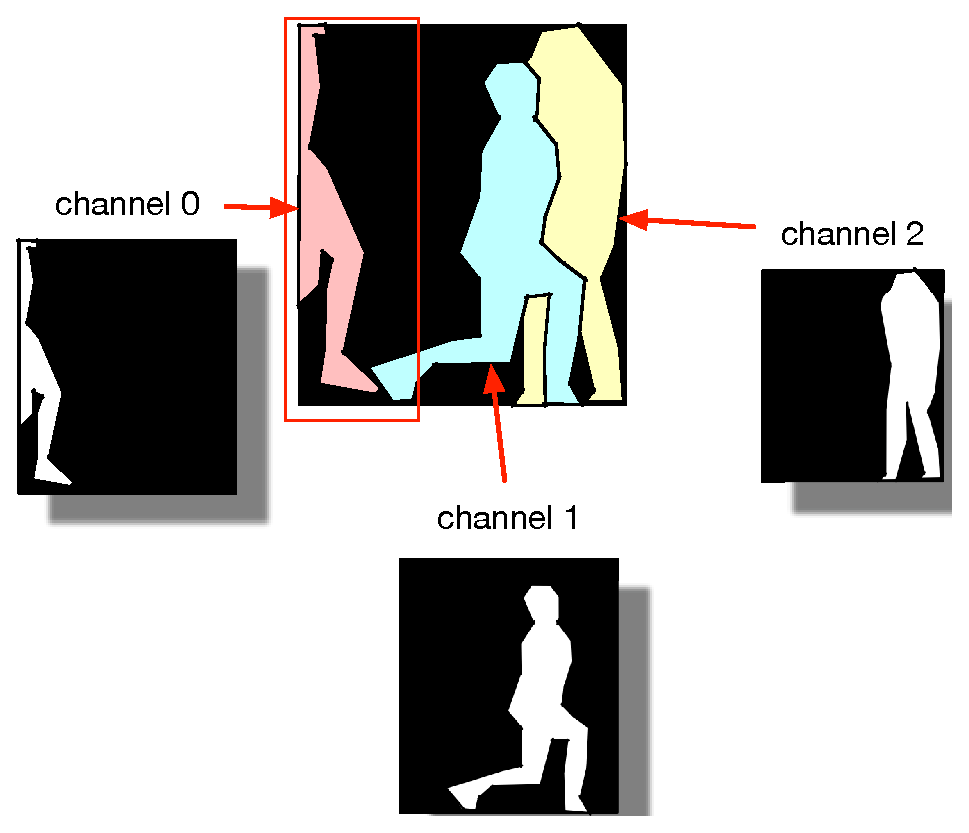
\includegraphics[scale=0.34]{instance_segmentation.eps}
	\caption{Channel-wise instance segmentation}
	\label{fig:chInsSeg}
\end{figure}

\section{本章小结}
